%% This is file `elsarticle-template-1-num.tex',
%%
%% Copyright 2009 Elsevier Ltd
%%
%% This file is part of the 'Elsarticle Bundle'.
%% ---------------------------------------------
%%
%% It may be distributed under the conditions of the LaTeX Project Public
%% License, either version 1.2 of this license or (at your option) any
%% later version.  The latest version of this license is in
%%    http://www.latex-project.org/lppl.txt
%% and version 1.2 or later is part of all distributions of LaTeX
%% version 1999/12/01 or later.
%%
%% Template article for Elsevier's document class `elsarticle'
%% with numbered style bibliographic references
%%
%% $Id: elsarticle-template-1-num.tex 149 2009-10-08 05:01:15Z rishi $
%% $URL: http://lenova.river-valley.com/svn/elsbst/trunk/elsarticle-template-1-num.tex $
%%
\documentclass[preprint,review,12pt]{elsarticle}

%% Use the option review to obtain double line spacing
%% \documentclass[preprint,review,12pt]{elsarticle}

%% Use the options 1p,twocolumn; 3p; 3p,twocolumn; 5p; or 5p,twocolumn
%% for a journal layout:
%% \documentclass[final,1p,times]{elsarticle}
%% \documentclass[final,1p,times,twocolumn]{elsarticle}
%% \documentclass[final,3p,times]{elsarticle}
%% \documentclass[final,3p,times,twocolumn]{elsarticle}
%% \documentclass[final,5p,times]{elsarticle}
%% \documentclass[final,5p,times,twocolumn]{elsarticle}


%%Use this packageto allow for accents 
\usepackage[utf8x]{inputenc}

%% The graphicx package provides the includegraphics command.
\usepackage{graphicx}
%% The amssymb package provides various useful mathematical symbols
\usepackage{amssymb}
%% The amsthm package provides extended theorem environments
%% \usepackage{amsthm}

%% The lineno packages adds line numbers. Start line numbering with
%% \begin{linenumbers}, end it with \end{linenumbers}. Or switch it on
%% for the whole article with \linenumbers after \end{frontmatter}.
\usepackage{lineno}

%% natbib.sty is loaded by default. However, natbib options can be
%% provided with \biboptions{...} command. Following options are
%% valid:

%%   round  -  round parentheses are used (default)
%%   square -  square brackets are used   [option]
%%   curly  -  curly braces are used      {option}
%%   angle  -  angle brackets are used    <option>
%%   semicolon  -  multiple citations separated by semi-colon
%%   colon  - same as semicolon, an earlier confusion
%%   comma  -  separated by comma
%%   numbers-  selects numerical citations
%%   super  -  numerical citations as superscripts
%%   sort   -  sorts multiple citations according to order in ref. list
%%   sort&compress   -  like sort, but also compresses numerical citations
%%   compress - compresses without sorting
%%
%% \biboptions{comma,round}

\journal{%Journal of Mathematical Psychology
}

\begin{document}

\begin{frontmatter}

%% Title, authors and addresses

\title{Bayesian Optimal Experimental Design for Generalized Linear Models.}

%% use the tnoteref command within \title for footnotes;
%% use the tnotetext command for the associated footnote;
%% use the fnref command within \author or \address for footnotes;
%% use the fntext command for the associated footnote;
%% use the corref command within \author for corresponding author footnotes;
%% use the cortext command for the associated footnote;
%% use the ead command for the email address,
%% and the form \ead[url] for the home page:
%%
%% \title{Title\tnoteref{label1}}
%% \tnotetext[label1]{}
%% \author{Name\corref{cor1}\fnref{label2}}
%% \ead{email address}
%% \ead[url]{home page}
%% \fntext[label2]{}
%% \cortext[cor1]{}
%% \address{Address\fnref{label3}}
%% \fntext[label3]{}


%% use optional labels to link authors explicitly to addresses:
%% \author[label1,label2]{<author name>}
%% \address[label1]{<address>}
%% \address[label2]{<address>}

\author{Manuel Villarreal, Carlos Vel\'{a}zquez and Arturo Bouzas}

\address{Mexico City, Mexico}

\begin{abstract}
%% Text of abstract
\end{abstract}

\begin{keyword}
Optimal experimental design \sep Generalized linear models \sep Psycophysics \sep Change point detection
%% keywords here, in the form: keyword \sep keyword

%% MSC codes here, in the form: \MSC code \sep code
%% or \MSC[2008] code \sep code (2000 is the default)

\end{keyword}

\end{frontmatter}

%%
%% Start line numbering here if you want
%%
\linenumbers

%% main text
\section{Introduction}
\label{S:1}

One of the main challenges in scientific research is the design of an experiment. A good experimental design will make the difference between finding an answer to our research question and wasting valuable resources like time and money.

When designing an experiment, often one starts by making decisions about the number of participants, how many and what values of our independent variable we should test or how many times should we test those values. Most of the time, these choices are made on the basis of previous research on the field. However, it might be the case that there is not enough information to make these decisions with confidence, or that the values that are commonly used, do not allow for strong conclusions. Optimal Experimental Design (OED) offers an alternative to solve this kind of problems through the formalization of the design problem.

OED allows us to re-interpret the problem of designing an experiment as a decision problem, in which the purpose is to maximize a utility function. This function is a numeric representation of our preference over the possible consequences of running an experiment. Therefore, the optimization of an experimental design requires us to have a formal interpretation of the purpose of the experiment.

The concept of optimizing an experimental design is not new to psychological research. There are already examples of design optimization in the literature \citep[e.g.][]{Myung2009,ZL2010}. Both of this examples discuss and demonstrate the advantages of OED for model comparison in psychology. 

In this paper, we will present a different approach where the problem is not to select between two models but to make inferences about the parameters of a single one.

%falta alguna cita despues de "widely used in psychophisics".
%falta alguna cita despues de "which has been used to model the relationship between a phisical stimulus and the probability of a given response".
In particular, we will present an example of OED in the context of Generalized Linear Models. These models are widely used in psychophysics. The problem that will be treated here is fairly new, however, the methodological aspects remain the same even with more straight-forward psychophysical experiments. In order to do this, we will use a particular parametrization of the logistic model which is primarily used in statistics.

\section{Optimal experimental design}

To apply the concepts of OED to a particular problem, first, we need to define the elements of the design space. This space is conformed by the variables that we can manipulate during the experiment, for example, the values that our independent variable might take or the weight (proportion of observations) assigned to each of those values. These elements are the ones that we can modify in order to optimize the design.

The second step would be to formalise the objective of the experiment. For example, in the case of a logistic model, we might want to find the values of our independent variable that minimize the variance of the model parameters, or we might be interested in the magnitude of the physical stimulus for which the probability of a response takes on a certain value. The formalization of the research question will define a utility function.

The last step is to specify the prior information that we have about the problem at hand. This last step can be carried out in two ways, first, we can try to optimize the experiment for a particular guess about the parameter values of the model of interest, or we could use a probability distribution to account for the uncertainty in the values that we are interested in. This last step is primarily important to the optimization process for generalized linear models, because the optimal design will depend on the values of the parameters.

% Perhaps i should present the formal arguments first a set of designs eta that belongs to...

Once we have defined the design space $\eta$, the objective of the experiment and the prior informartion $p(\theta)$, the expected utility of a design is represented by the following equation:
\begin{equation}
U(\eta)=\int \int U(\eta,y,\theta)p(\theta|y,\eta)p(y|\eta) d\theta dy
\label{eu}
\end{equation}
Therefore, finding the experimental design that is optimal given a utility function, reduces to the problem of finding the values for the variables in $\eta$ for which equation \ref{eu} takes it's maximum value.

Many utility functions have been proposed for both linear and non-linear design problems, however, as was previously mentioned, the choice of a utility function depends on the research question. For example, \cite{Myung2009} utilizes the sum of squered errors between the data generated by a model and the predictions of a competing one given an expeirmental design. This is because, the objective is to find a design that can discriminate the predictions of the two. On the other hand, \cite{ZL2010} choose a utility function based on the Bayes Factor. Both of this functions will have their advantages, nontheless, the first utility emphasizes disciminability of model's predictions, while the second one aims for a design in which the data generating model is more likely.

When the objective of the experiment is to make an inference about the parameters of a generalized linear model, some authors \citep[e.g.][]{Ber1979} have proposed to consider the gain in Shanon's Information as a utility function. In this case, the objective is to find the design $\eta$ that maximizes the expected gain in Shanon Information, or equvalently, maximizes the Kullback-Leibler divergence between the posterior and prior distribution. With this function, the expected utility of an experimental design is represented by the following equation:
\begin{equation}
U(\eta)=\int \int log\frac{p(\theta|y,\eta)}{p(\theta)} p(y,\theta |\eta) d\theta dy
\label{klu}
\end{equation}
The prior distribution in the denominator of the logarithm can be droped as it does not depend on the experimental design, therefore, the optimal design will be the one that maximizes:
\begin{equation}
U(\eta)=\int \int log \{p(\theta|y,\eta)\} p(y,\theta |\eta) d\theta dy
\label{egShanon}
\end{equation}
Which is the posterior expected Shanon information.

When dealing with generalized linear models, the posterior distribution of the parameter vector $\theta$ is not always tractable, however, in the literature of design optimization it is common to use the following aproximation to the posterior distribution
\begin{equation}
\theta|y,\eta \sim N\left(\hat{\theta},[nI(\hat{\theta},\eta)]^{-1}\right)
\label{Naprox}
\end{equation}
Where $I(\hat{\theta},\eta)$ denotes the observed fisher information matrix given an experimental design and $\hat{\theta}$ is the maximum likelihood estimate of $\theta$. Even with this, the marginal distribution of the data ($p(y|\eta)$) in equation \ref{eu} also needs to be aproximated, however, when the posterior utility only depends on $y$ through some constistent estimate of $\hat{\theta}$, a further approximation is to take the predictive distribution of  $\hat{\theta}$ to be the prior distribution \cite{chalar1989}.

With both aproximations, the value of $U(\eta)$ is:
\begin{equation}
U(\eta)=-\frac{k}{2}log(2\pi)-\frac{k}{2}+\frac{1}{2} \int log \{det[nI(\theta,\eta)]\} p(\theta) d\theta
\label{aproxu1}
\end{equation}
Equation \ref{aproxu1} gives the exact expected utility of an esperimental design. However, one could drop the constant and multiplier terms giving the following form:
\begin{equation}
\phi(\eta)= \int log \{det[nI(\theta,\eta)]\} p(\theta) d\theta
\label{crit1}
\end{equation}
The function $\phi(\eta)$ is known as a design critirion. An optimal design would be the one maximizing equation \ref{crit1}, nontheless, it is worth noting that this relies on the normal approximation to the posterior distribution in \ref{Naprox}, therefore, for small smaples there are some constraints that help to assure normality (see \cite{CLCH2002}).

% Why is is detecting changes important for an organism?
% 
% Change detection in probabilistic series.
% 
% Arising problems with experimental design.


% Elements:
% 
% Design space: what are the elements of the experimental design that we want to optimize
% Utility Function: function that maps points on the design space to the real numbers, this function should reflect the objective of the experiment, for example if we want to discriminate between two cognitive models, the utility function should assign a greater value to an experimental design for which the models give different predictions that to designs for which the predictions of the models are indistinguishable from one another.

\section{OUTLINE}

% EXAMPLE CITING Maecenas \cite{Smith:2012qr} fermentum \cite{Smith:2013jd} %

%EXAMPLE ITMES and  ENUMERATING
%\begin{itemize}
%\item Bullet point one
%\item Bullet point two
%\end{itemize}
%\begin{enumerate}
%\item Numbered list item one
%\item Numbered list item two
%\end{enumerate}

%%%% EXAMPLE TABLE
%\begin{table}[h]
%\centering
%\begin{tabular}{l l l}
%\hline
%\textbf{Treatments} & \textbf{Response 1} & \textbf{Response 2}\\
%\hline
%Treatment 1 & 0.0003262 & 0.562 \\
%Treatment 2 & 0.0015681 & 0.910 \\
%Treatment 3 & 0.0009271 & 0.296 \\
%\hline
%\end{tabular}
%\caption{Table caption}
%\end{table}

%%%% EXAMPLE Labeled Equiation
%\begin{equation}
%\label{eq:emc}
%e = mc^2
%\end{equation}

\section{Optimal Experimental Design: Example}
\label{S:2}

Why is is detecting changes important for an organism?

Change detection in probabilistic series.

Arising problems with experimental design.

Research question and its statistichal interpretation

Assumtion about the relationship between a subjects response the dependent variable under study

Design space for this problem and how to reduce the dimensionality of the space by assuming experimental constraints.

Utility function and its relationship with the objective of the experiment

Arising problems with utility function and the proposed response function. Bayesian solution, assigning a prior distribution to the parameters, the less research in a field the more difficult it is to assign an informative prior, however, we could use other cognitive models in order to propose a prior distribution. 
 % EXAMPLE Reference of a labeled Section \ref{S:1}
\subsection{Using a model to generate prior distributions}

Using the prior distribution, the utility function and the definition of a design space we can otimize the experimental design in this case we are looking for \begin{math}\mathbf{\delta\theta}^{*}\end{math} that maximizes the following equation:

\begin{equation}
U(\mathbf{\delta\theta}^{*})=\max_{\delta\theta} \int_{\mathbf{\beta}} log(det(I(\beta|\mathbf{\delta\theta}))) \pi(\mathbf{\beta}) d\mathbf{\beta}
\end{equation}

The previous integral can be approximated via Monte Carlo sampling

\section{Results}
\label{S:3}

\subsection{Consruction of the prior distribution}

Prior over model parameters(Gallistel et al 2014)
Results
Constructing the prior: we take a multivariate normal distribution with mean and covariance equal to the unbiased estimators for both parameters.


\subsection{Optimal design}

\begin{figure}
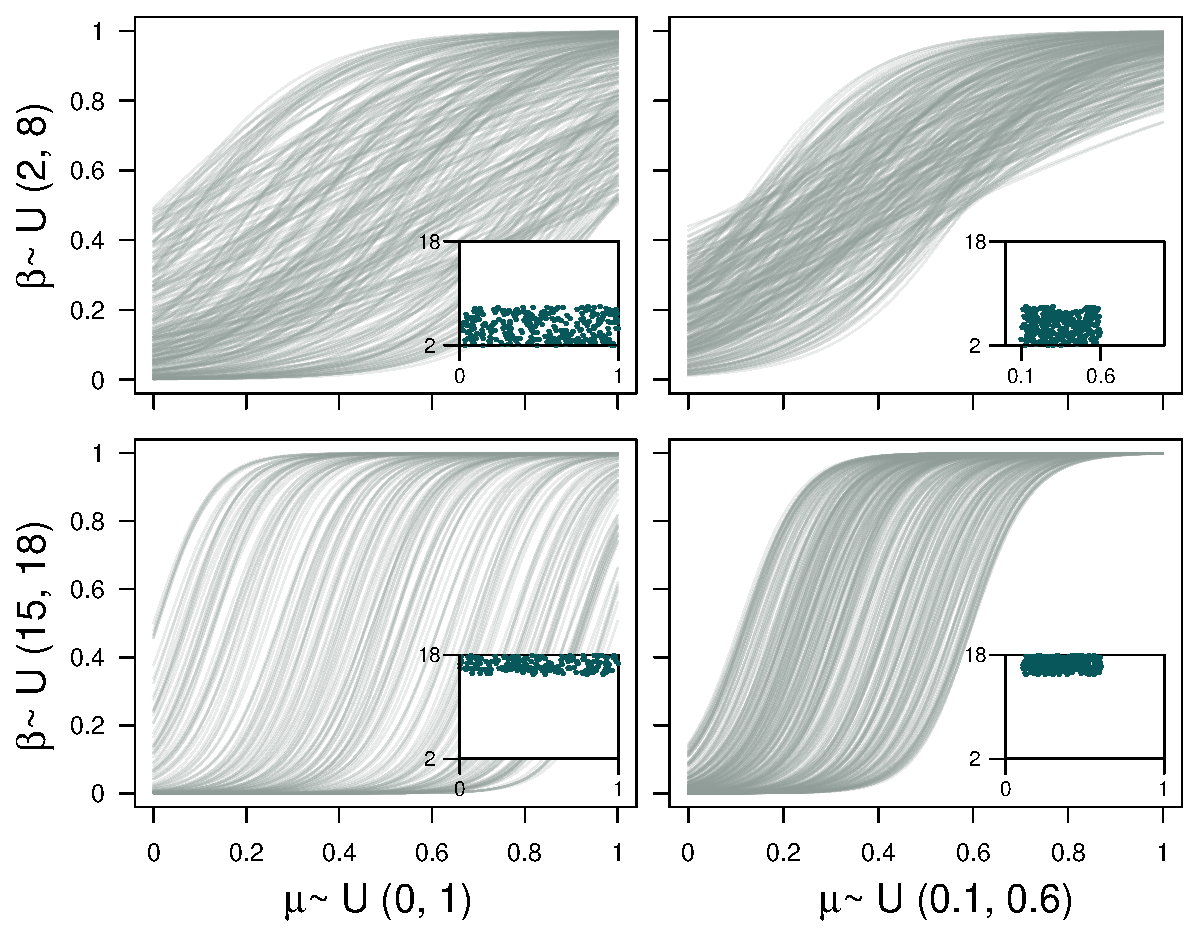
\includegraphics[width=\textwidth]{Prior_and_Predictive.pdf}
\caption{Prior and predictive prior distributions.}
\label{fig:ppd}
\end{figure}

\begin{figure}
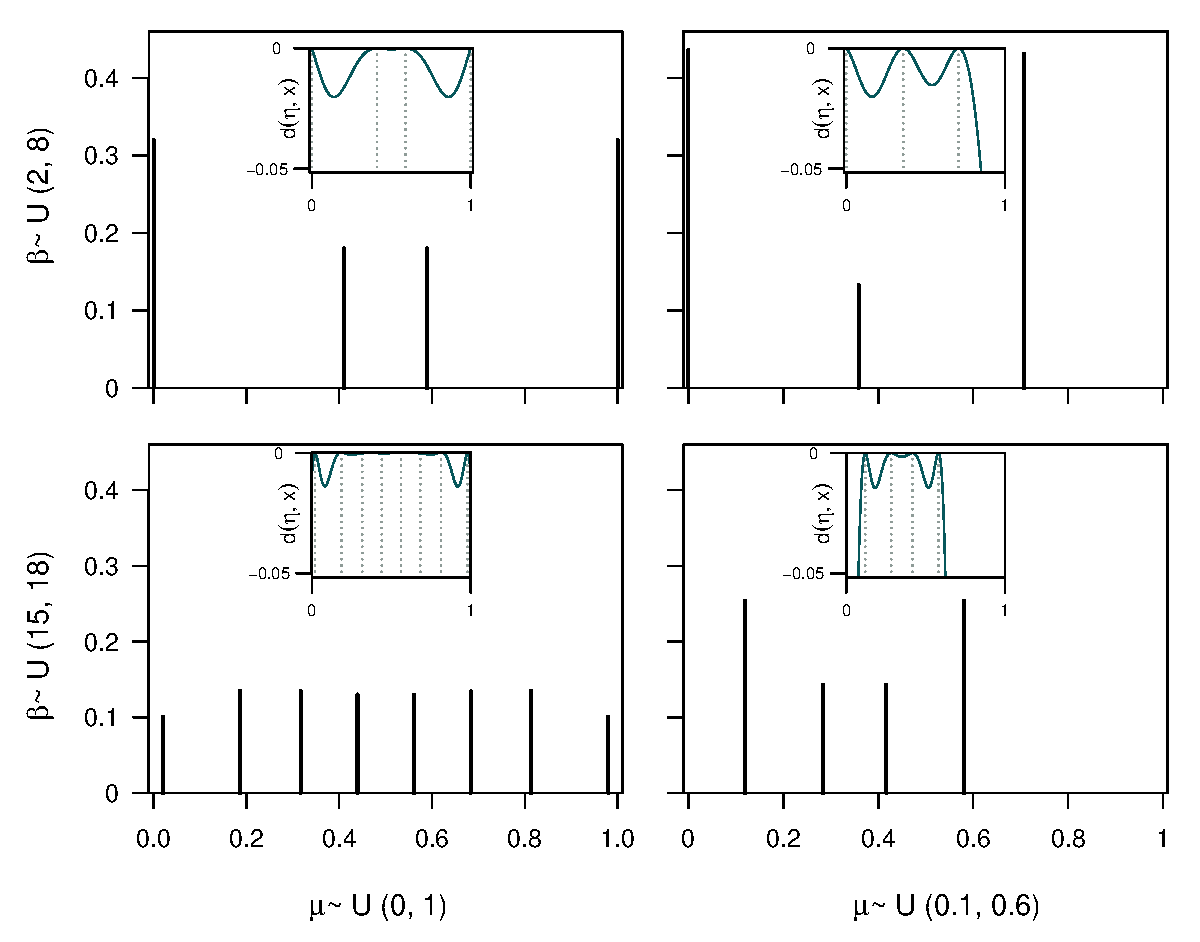
\includegraphics[width=\textwidth]{Support_detadx.pdf}
\caption{Optimal experimental designs and directional derivatives.}
\label{fig:detadx}
\end{figure}

\begin{figure}
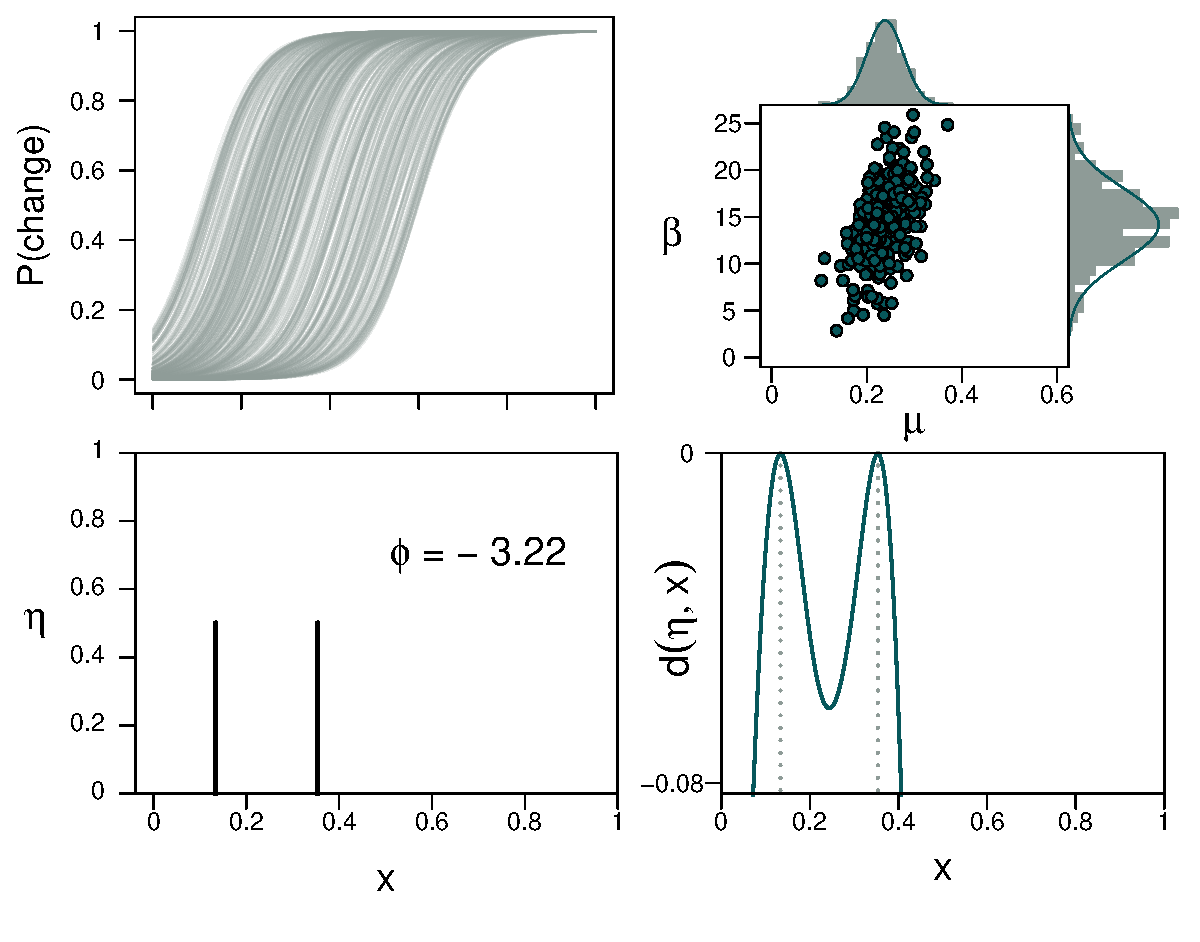
\includegraphics[width=\textwidth]{Joint_Normal.pdf}
\caption{Informative prior distribution, prior predictive, optimal design and directional derivative.}
\label{fig:jn}
\end{figure}

Aproximating the utility function (integral) throught Monte Carlo simulation 
Utility aproximation for 2 Design points 

the approximation returns a smooth curve over the 2 point design space.

\section{Discussion}
\label{S:4}

Optimal design for the example
Properties of the most useful points (they land on the points of the curve where the steepness changes most dramatically)

Advantages of Optimal Design

Using models to generte prior distributions.

%% The Appendices part is started with the command \appendix;
%% appendix sections are then done as normal sections
%% \appendix

%% \section{}
%% \label{}

%% References
%%
%% Following citation commands can be used in the body text:
%% Usage of \cite is as follows:
%%   \cite{key}          ==>>  [#]
%%   \cite[chap. 2]{key} ==>>  [#, chap. 2]
%%   \citet{key}         ==>>  Author [#]

%% References with bibTeX database:

\section*{References}
\bibliographystyle{elsarticle-harv}
\biboptions{authoryear}
\bibliography{OD_Psychophisics}

%% Authors are advised to submit their bibtex database files. They are
%% requested to list a bibtex style file in the manuscript if they do
%% not want to use model1-num-names.bst.

\end{document}

%%
%% End of file `elsarticle-template-1-num.tex'.